\scanpage{31}
\reversemarginpar
\margin{\figure{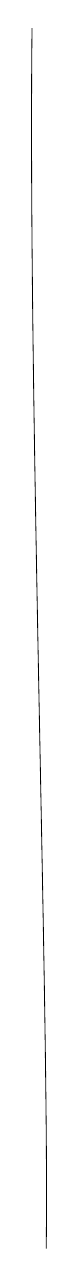
\begin{tikzpicture}[x=1cm,y=1cm]
\draw[line width=.3pt] (0,-.8) .. controls (-.05,-5.4) and (.22,-13.4) .. (.18,-16.3);
\end{tikzpicture}}}
\normalmarginpar
\uline{Théorème} 2.1.1. Soit $f:S'\handwritten{\longrightarrow}S$ un morphisme universellement localement \uline{$L$}-\unsure{1|l}-asphérique (SGA 4 XV \handwritten{1.11}), par exemple (SGA\handwritten{4}XV \handwritten{\unsure{2.1|2.2}}) un morphis\unsure{m} lisse, ou tel que $\deleted{\unsure{X|S}}\handwritten{S'}$ soit isomorphe à la limite \inserted{projective} d'un systême projectif \inserted{filtrant} de $S$-schémas lisses $S'_i$ à morphismes de transition affines\deleted{\unsure{,}} (SGA 4 XV \handwritten{1.13\inserted{(ii)}})
% The right edge clips the last m of morphisme; no absent terminal e is supplied.

Soi\inserted{en}t $g:X\handwritten{\longrightarrow}S$ un morphisme de schémas, d'où un carré car\unsure{\deleted{ét}té|\deleted{té}ét}sien
\diagram{\begin{tikzpicture}
\node[inner sep=0pt] (square) {\begin{tikzcd}[ampersand replacement=\&,row sep=2.2em,column sep=4em]
X \handwritten{\arrow[d,"g"']} \& X' \handwritten{\arrow[l,"f'"']} \handwritten{\arrow[d,"g'"]} \\
S \& S'\handwritten{\arrow[l,"f"']}\rlap{,}
\end{tikzcd}};
\draw[line width=.3pt] ([xshift=-4pt,yshift=-4pt]square.west) -- ([xshift=-2pt,yshift=-13pt]square.west);
\draw[line width=.3pt] ([xshift=0pt,yshift=-10pt]square.west) .. controls ([xshift=2pt,yshift=-14pt]square.west) and ([xshift=1pt,yshift=-17pt]square.west) .. ([xshift=1pt,yshift=-19pt]square.west);
\end{tikzpicture}}

$G$ un \inserted{ind-\uline{$L$}-} champ sur $X$ \inserted{\handwritten{($\overline{\text{\uline{V}}}$ 5\quad),}} \deleted{dont les faisceaux d'automorphismes sont des ind-\uline{$L$}-faisceaux} $G'=f'^*(G)$ le champ image inverse sur $X'$.

\begin{enumerate}[label=\alph*)]
\item Si \deleted{$S$ et $S'$ sont strictement locaux et} $f$ est un morphisme \deleted{strictement} \uline{local} de schémas strictement locaux, alors le foncteur
\[
\handwritten{G(X)\longrightarrow G'(X')}
\]
est une équivalence de catégories.

\item Si $g$ est cohérent(i.e. quasi-compact et quasi-séparé) alors le morphisme de champs ``de changement de base''
\[
f^{\handwritten{'}}(g_{\handwritten{*}}(G))\handwritten{\longrightarrow}g'_{\handwritten{*}}(f'^{\handwritten{*}}(G))\deleted{\handwritten{\unsure{=g_{\unsure{*|<}}'|g_{\unsure{*|<}}'|=g_{\unsure{*|<}},|g_{\unsure{*|<}},}}}
\]
est une équivalence de champs sur $S'$.
\end{enumerate}

\reversemarginpar
\margin{\figure{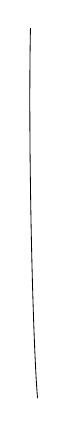
\begin{tikzpicture}[x=1cm,y=1cm]
\draw[line width=.3pt] (0,-.5) .. controls (-.03,-2.0) and (.03,-4.5) .. (.09,-5.2);
\end{tikzpicture}}}
\normalmarginpar
\uline{Corollaire} 2.1.2. Soient $k$ un corps séparablement clos, $k'$ une extension séparablement close de $k$, $X$ un $k$-schéma, $X'=X\handwritten{\otimes}_k k'$, alors pour tou\unsure{t} \deleted{champ $G$} ind-\uline{$L$}-champ $G$ sur $X$, désignant par $G'$ son image inverse sur $X'$, le foncteur
\[
\handwritten{G(X)\longrightarrow G'(X')}
\]
est une équivalence de catégories.

O\unsure{\(\mathbb{n}\)|\deleted{p}n|\deleted{n}p} sait en effet (SGA 4 XVI\quad\quad) que $\operatorname{Spec}(k')\handwritten{\longrightarrow}\operatorname{Spec}(k)$ est universellement localement \uline{$L$}-1-asphérique.

Démonstration. On prouve a) par référence à SGA 4 XVI (nouvelle édition !)\inserted{\handwritten{et à $\overline{\text{\uline{V}}}$ - -}}, et b) en se ramenant à a) par des lemmes 2.1.7.2 et 2.1.7.4 renumérotés.
\margin{\handwritten{En tout, ça devrait faire 3 pages au \unsure{Ch.p|Chap.} $\overline{\text{\uline{VII}}}$ au maximum, -- mais il y \unsure{aurait|aura} renvois au Ch.p $\overline{\text{\uline{V}}}$.}}
% archive sheet number: 30

